\newpage
\subsection{Defining Classes}
\texHeader
\hypertarget{static:classes tex}{}

\begin{itemize}

\item[$\blacktriangleright$] Right click on \texttt{LearningBoxLanguage} and create your first eclass model by going to ``New/EClass.'' Name it \texttt{Box}.

\vspace{0.5cm}

\item[$\blacktriangleright$] The class editor should have automatically appeared. Currently, it's empty; Lets add the first two EAttributes of our program,
\texttt{name} and \texttt{stringRep}. Both are \texttt{EString} types (Fig.~\ref{fig:boxDeclaration}).

\vspace{0.5cm}

\begin{figure}[htbp]
	\centering
  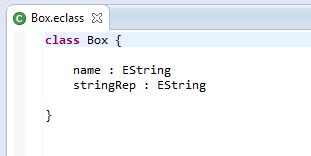
\includegraphics[width=0.4\textwidth]{eclipse_classBoxDeclaration}
	\caption{Newly created box class}
	\label{fig:boxDeclaration}
\end{figure} 

\item[$\blacktriangleright$] Create two more classes in your model the same way, \texttt{Partition} and \texttt{Card}.

\vspace{0.5cm}

\item[$\blacktriangleright$] In \texttt{Partition}, add two \texttt{EInt} datatypes, \texttt{index} and \texttt{partitionSize}.

\vspace{0.5cm}

\item[$\blacktriangleright$] In \texttt{Card}, create three \texttt{EString}s, \texttt{back}, \texttt{face} , and \texttt{partitionHistory}.

\vspace{0.5cm}

\item[$\blacktriangleright$] If you've done everything correctly, the key areas of your workspace should now resemble Fig.~\ref{fig:workspaceClassAttributes}.

\vspace{0.5cm}

\item[$\blacktriangleright$] Closing message

\newpage

\vspace*{3cm}

\begin{figure}[htbp]
	\centering
  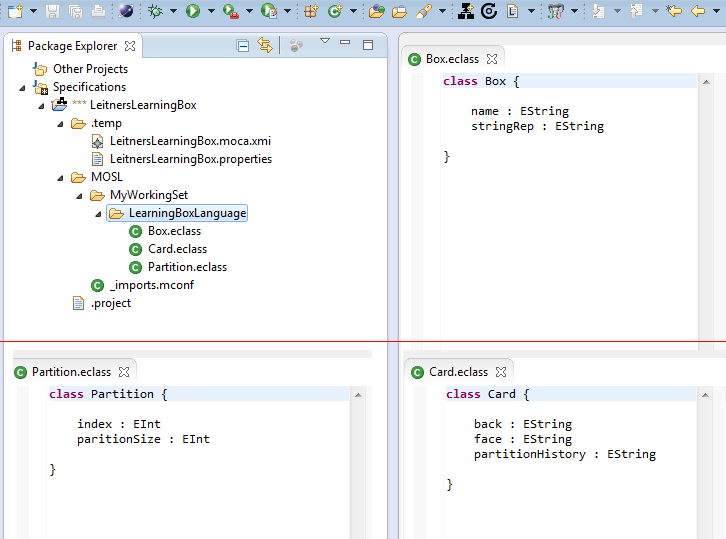
\includegraphics[width=1\textwidth]{eclipse_workspaceClassesAttributes}
	\caption{Declaration of classes and attributes}
	\label{fig:workspaceClassAttributes}
\end{figure} 

\fancyfoot[R]{$\triangleright$ \hyperlink{static:references tex}{Next}}

\end{itemize}
